\documentclass[a4paper]{article}
\usepackage{mystyle}

\begin{document}

\customtitle{Fluctuation Strength Test Battery}

\section{Introduction}

This document details a series of test that will be used to validate model
implementations of fluctuation strength. These tests will be based on the
reference value of fluctuation strength and its the parametric dependencies. For
all the tests a sampling frequency $f_s = 44100 $ Hz will be used.

\section{Reference Value}

An AM (amplitude-modulated) tone ($f_c = 1$ kHz, $f_m = 4$ Hz, $m_d = 1$,
SPL $=60$ dB) serves as the reference value for fluctuation strength, with a
value of 1 vacil assigned to it. As so, the model implementation must comply
with this requisite.

\section{Tests}

This section details the specific tests that the model must pass to be
considered adequate. According to the type of input stimuli different tests
will be specified, starting with AM tones and then expanding to FM
(frequency-modulated) tones and AM BBN (broadband noise).

\subsection{AM Tones}

\subsubsection{Modulation Frequency}

The most characteristic attribute of fluctuation strength is its bandpass
response with regard to the variation of the modulation frequency (Figure
\ref{fig:flucstrenvmodfreq}b). As so, this particular plot will be reproduced
using the input stimuli whose parameters are shown on Listing
\ref{lst:amparamsfmplot}.

\begin{lstlisting}[
    style=MATLAB-editor,
    caption={AM tones parameters modulation frequency plot},
    label={lst:amparamsfmplot}
]
fc  = 1e3;
md  = 1;
SPL = 70;
fs  = 44100;
N   = 81920;
FMs = [0.25 0.50 1.00 2.00 4.00 8.00 16.00 32.00];
\end{lstlisting}

\begin{figure}[ht]
    \centering
    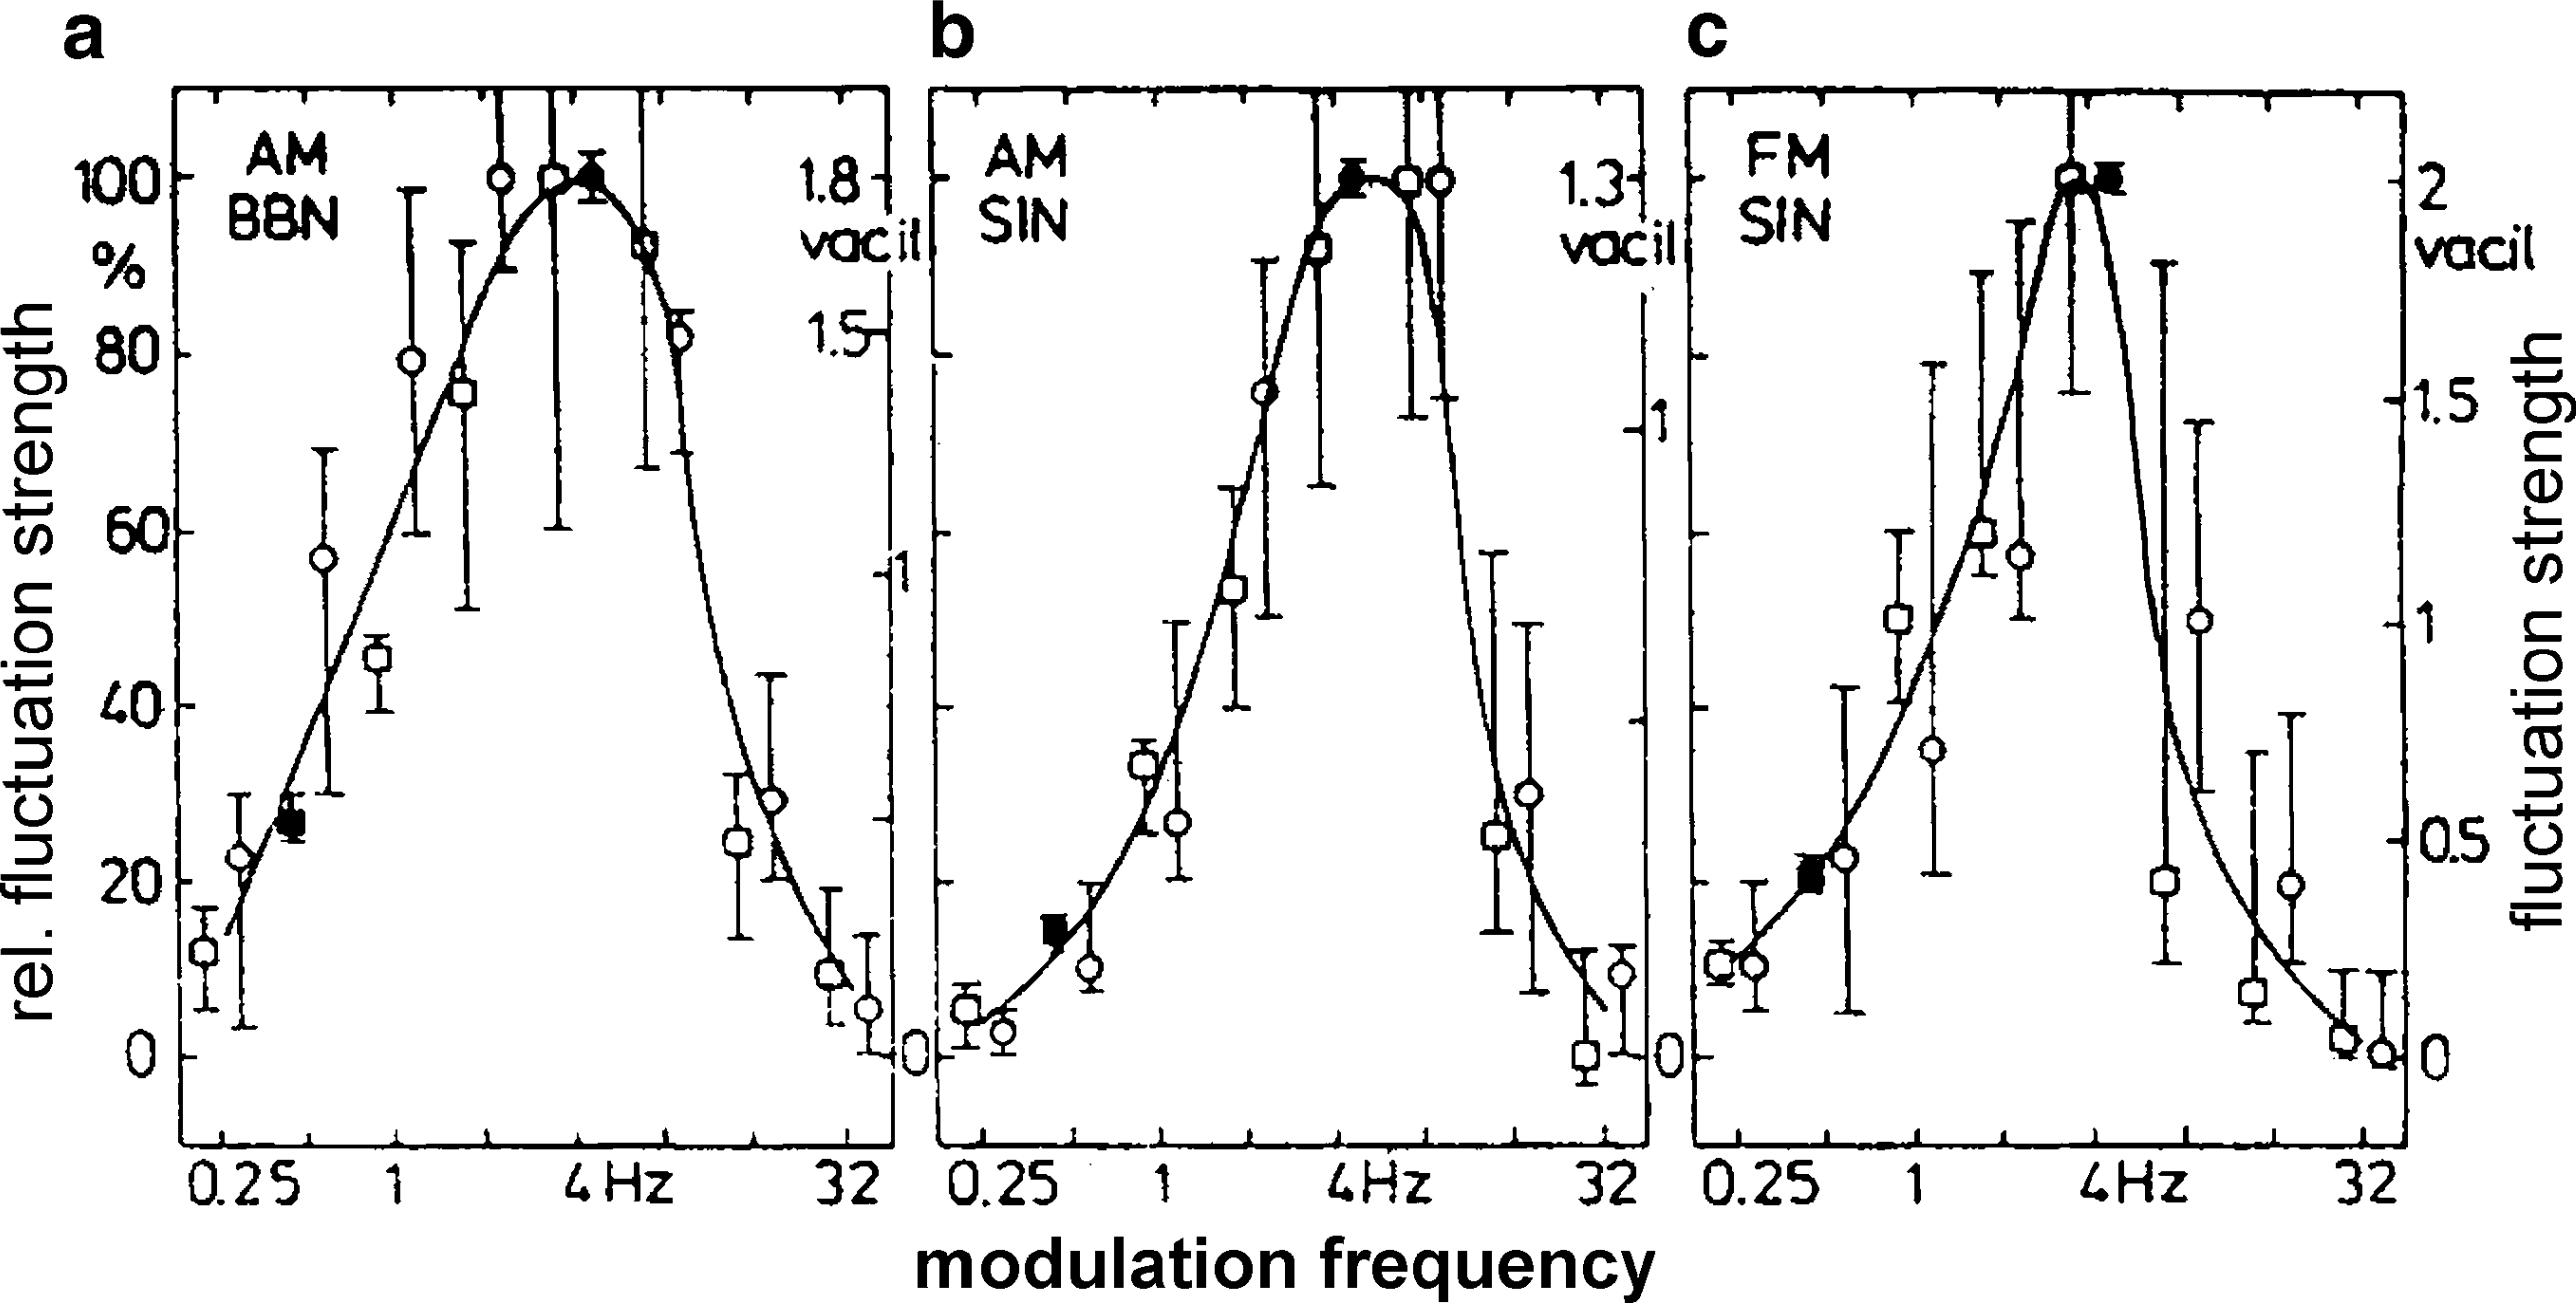
\includegraphics[height=8cm]
        {book/img/Mueller2012Handbook-FluctuationStrengthVsModulationFrequency}
    \caption{Fluctuation strength of three modulated sounds as a function of
        modulation frequency. (a) Amplitude-modulated broad-band noise of 60-dB
        SPL and 40-dB modulation depth; (b) amplitude-modulated 1-kHz tone of
        70-dB SPL and 40-dB modulation depth; (c) frequency-modulated pure tone
        of 70-dB SPL, 1500-Hz center frequency and $\pm$ 700-Hz frequency
        deviation; \cite[pp. 248]{Fastl2007Psychoacoustics}}
    \label{fig:flucstrenvmodfreq}
\end{figure}

\bibliographystyle{plainnat}
\bibliography{../References}

\end{document}
